% arara: pdflatex: { shell: true }
% arara: xelatex: { synctex: 1, shell: yes }
% arara: lualatex: { shell: true, interaction: nonstopmode }
\documentclass{article}	
\usepackage{minted}
\usemintedstyle{xcode} % Optional: Set a code style (vs is just an example)
\usepackage{hyperref}
\usepackage{graphicx}
\usepackage{pdfpages}

\title{Record}
\author{Name}
\date{2023-12-28}

\begin{document}
  
\includepdf[pages={1}]{./Assets/bob.pdf}
  \newpage
  \tableofcontents
  \newpage

  \section{Simple Html Page}
    \subsection*{Aim}
    \begin{itemize}
      \item Design a webpage for your department.
      \item Utilize paragraphs and lists.
      \item Create links of the words Wifi and LAN to their respective wikipedia pages
      \item Insert an image that redirects to the college website
      \item Change the background color and create a link at the bottom to return to the top
    \end{itemize}

    \subsection*{Code}
      \inputminted[frame=lines, linenos, breaklines, breakanywhere, numberblanklines=false]{html}{./prog_1/index.html}

    \subsection*{Output}
    \begin{figure}[h!]
    \centering
    
\includegraphics[width=0.8\textwidth]{./Assets/p0101.png}
    \end{figure}
  \newpage

  \section{Time Table}
    \subsection*{Aim}
    \begin{itemize}
      \item Design the class time table in HTML using table tag
    \end{itemize}

    \subsection*{Code}
      \inputminted[frame=lines, linenos, breaklines, breakanywhere, numberblanklines=false]{html}{./prog_2/index.html}

    \subsection*{Output}
    \begin{figure}[h!]
    \centering
    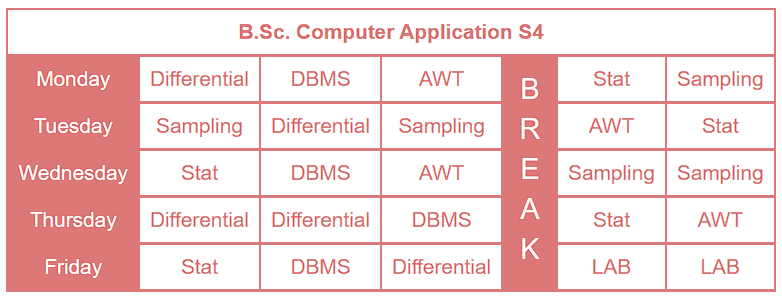
\includegraphics[width=0.8\textwidth]{./Assets/p0201.png}
    \end{figure}
  \newpage

  \section{CSS}
    \subsection*{Aim}
    \begin{itemize}
      \item Utlize inline CSS for appending styles to html elements
      \item Utilize an external CSS Stylesheet
    \end{itemize}

    \subsection*{Code}
      \inputminted[frame=lines, linenos, breaklines, breakanywhere, numberblanklines=false]{html}{./prog_3/index.html}
      External Stylesheet
      \inputminted[frame=lines, linenos, breaklines, breakanywhere, numberblanklines=false]{css}{./prog_3/styles.css}

    \subsection*{Output}
    \begin{figure}[h!]
    \centering
    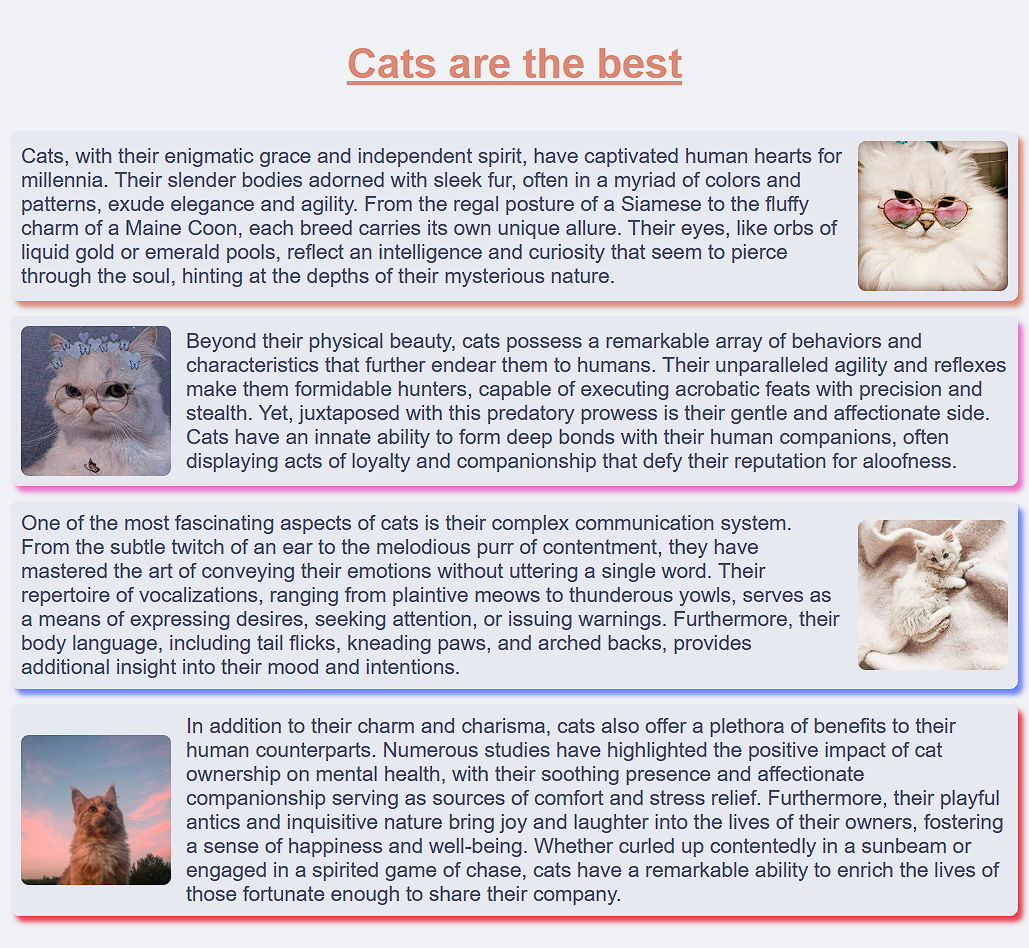
\includegraphics[width=1.0\textwidth]{./Assets/p0301.png}
    \end{figure}
  \newpage
\end{document}
